\documentclass[11pt,tikz,border=3.14mm]{standalone}
\usepackage{xcolor}
\definecolor{r1}{HTML}{FF8674}
\definecolor{b1}{HTML}{17ABDD}
\definecolor{p1}{HTML}{D4B6D6}
\definecolor{g1}{HTML}{70E2CB}
\definecolor{o1}{HTML}{DFA743}
\usepackage{mathptmx}
\usepackage{siunitx}

\begin{document}
  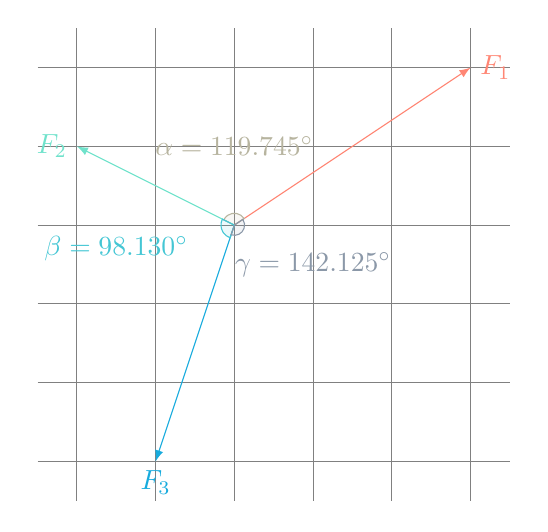
\begin{tikzpicture}
  % 网格
  \draw [gray] (-2.5,-3.5) grid (3.5,2.5);
  
  % 三个作用力
  \draw [-latex,r1] (0,0) -- (3,2) node [right] {$F_1$};
  \draw [-latex,g1] (0,0) -- (-2,1) node [left] {$F_2$};
  \draw [-latex,b1] (0,0) -- (-1,-3) node [below] {$F_3$};
  
  %角度标注
  \draw [color=r1!50!g1,fill=r1!50!g1,fill opacity=0.1] (0,0) -- (33.690067525979785:0.15) arc (33.690067525979785:153.434948822922:0.15) --cycle;
  \draw [color=g1!50!b1,fill=g1!50!b1,fill opacity=0.1] (0,0) -- (153.434948822922:0.17) arc (153.434948822922:251.565051177078:0.17) --cycle;
  \draw [color=b1!50!r1,fill=b1!50!r1,fill opacity=0.1] (0,0) -- (-108.43494882292202:0.13) arc (-108.43494882292202:33.69006752597979:0.13) --cycle;

  %角度数值
  \draw[color=r1!50!g1] (0,1) node {$\alpha = \ang{119.745}$};
  \draw[color=g1!50!b1] (-1.5,-0.3) node {$\beta = \ang{98.130}$};
  \draw[color=b1!50!r1] (1,-0.5) node {$\gamma = \ang{142.125}$};

  \end{tikzpicture}
\end{document}